
\documentclass[sigconf,review,anonymous]{acmart}
\settopmatter{printacmref=false}
\renewcommand\footnotetextcopyrightpermission[1]{}
\pagestyle{plain}

\acmConference[ASE '26]{Proceedings of the 41st IEEE/ACM International Conference on Automated Software Engineering}{October 12--16, 2026}{Munich, Germany}
\acmBooktitle{Proceedings of the 41st IEEE/ACM International Conference on Automated Software Engineering (ASE '26), October 12--16, 2026, Munich, Germany}
\acmYear{2026}
\copyrightyear{2026}
\setcopyright{none}

\usepackage{amsmath}
\usepackage{booktabs}
\usepackage{enumitem}
\usepackage{graphicx}
\usepackage{microtype}
\usepackage{multirow}
\usepackage{tabularx}
\usepackage{xcolor}
\usepackage{tikz}
\usetikzlibrary{arrows.meta,positioning,fit,calc,shapes.geometric,shapes.multipart,backgrounds,matrix}

\newcommand{\ccbench}{\textsc{Capability-Clash}}
\newcommand{\pp}{\,pp}
\newcommand{\agent}[1]{\textsc{#1}}

%--- colour palette ---
\definecolor{clrRLedge}{RGB}{37,99,180}
\definecolor{clrRLfill}{RGB}{219,234,254}
\definecolor{clrExecedge}{RGB}{22,123,80}
\definecolor{clrExecfill}{RGB}{209,250,229}
\definecolor{clrAuditedge}{RGB}{185,28,28}
\definecolor{clrAuditfill}{RGB}{254,226,226}
\definecolor{clrRewardedge}{RGB}{180,100,0}
\definecolor{clrRewardfill}{RGB}{254,237,192}
\definecolor{clrZoneedge}{RGB}{100,116,139}
\definecolor{clrZonefill}{RGB}{248,250,252}
\definecolor{clrSweetfill}{RGB}{187,247,208}
\definecolor{clrSatfill}{RGB}{226,232,240}

\tikzset{
  figflow/.style={-{Latex[length=2.4mm,width=1.7mm]}, line width=0.5pt},
  rlnode/.style={draw=clrRLedge, fill=clrRLfill, rounded corners=3pt, align=center, line width=0.6pt},
  execnode/.style={draw=clrExecedge, fill=clrExecfill, rounded corners=3pt, align=center, line width=0.6pt},
  auditnode/.style={draw=clrAuditedge, fill=clrAuditfill, rounded corners=3pt, align=center, line width=0.85pt},
  rewardnode/.style={draw=clrRewardedge, fill=clrRewardfill, rounded corners=3pt, align=center, line width=0.6pt},
  statenode/.style={draw=clrZoneedge, fill=clrZonefill, rounded corners=4pt, align=center, line width=0.6pt}
}

\begin{document}

\title[Capability-Clash]{Capability-Clash: Hard Semantic Floors, Precision-over-Scale Inversion, and Reward Corruption in LLM Code Repair}

\author{Anonymous Author(s)}
\affiliation{\institution{Under Double-Blind Review}}
\email{anonymous@anonymous.invalid}

\begin{abstract}
Every single one of 72 test-passing repairs produced by four state-of-the-art LLMs on an adversarial code-repair benchmark is semantically incomplete. This means the standard RL training signal — test-suite pass rate — is not merely noisy on adversarially-designed tasks: it is systematically and completely wrong. We present \ccbench{}, a 1{,}184-run controlled benchmark (37 tasks $\times$ 8 strategies $\times$ 4 models) targeting the seeded-repair regime — single-site mutations injected into five real repositories where the agent must revert an unknown change across five semantically distinct mutation families (Python, Node.js, PHP). All 37 tasks are evaluated across four models from two providers (gpt-4.1-mini, gpt-4.1-nano, claude-haiku-4-5, claude-opus-4-6). The benchmark yields two findings that jointly reframe RL-based code repair evaluation.

\textbf{Finding 1 — hard semantic floor and precision-over-scale inversion.}
All models plateau at low pass rates (Nano 7.8\%, Opus 8.8\%, Mini 16.6\%, Haiku 19.3\%), with 21/37 tasks failing for all four models (56.8\% hard floor). The floor persists across task subsets: on the 30 core-set Python/Node.js tasks (excluding the four PHP/Appwrite tasks and three tasks with multi-file targets), 20/30 tasks (66.7\%) fail both mini and nano on all strategies. Within the Anthropic family, a statistically significant \emph{precision-over-scale inversion} occurs: the smaller Haiku (19.3\%) outperforms the larger Opus (8.8\%) by +10.5\pp{} ($z=3.67$, $p<0.001$). Within OpenAI, the expected direction holds: Mini (16.6\%) $>$ Nano (7.8\%). The cross-provider asymmetry — inversion within Anthropic, normal scaling within OpenAI — is itself informative: it reveals that instruction-following precision (Haiku's profile) outperforms raw scale (Opus) on surgical seeded-repair tasks, with models showing complementary task profiles ($\kappa = 0.44$ between Haiku and Opus). The mechanism is \emph{repair decisiveness}: Haiku passes in 0.51 repair rounds on average — finding the surgical fix on the first attempt — while floor-tier models require 1.04 rounds even on tasks they eventually solve. The floor is not an artifact of closed-source API models: an open-weight 3B model (qwen2.5-coder:3b, Ollama) achieves \textbf{0/103 = 0.0\%} across 25+ tasks from 4 repositories (103 runs, 4 strategies), lower than every canonical model on every matched task subset, confirming the floor is structural.

\textbf{Finding 2 — reward signal failure.}
100\% of 72 test-passing repairs are semantically incomplete per post-hoc audit: an RL agent trained here learns to produce plausible-but-wrong patches reliably. A reference-free LLM judge achieves F1$=$0.615; augmenting with the ground-truth patch yields F1$=$0.993, \emph{crossing} the F1$\geq$0.8 RL-training viability threshold. Counterintuitively, gpt-4.1-mini $+$ GT (F1$=$0.993) outperforms gpt-4.1 $+$ GT (F1$=$0.917): calibration beats raw scale in verification. As a judge calibration check, the same reference-free judge rates 96.7\% of SWE-bench Lite gold patches as \texttt{COMPLETE} ($\text{RCG}_{\text{field}} \approx 0.97$) — confirming the 100\% \ccbench{} disagreement rate reflects adversarial task design, not judge bias.

Together, these findings yield a \emph{four-part routing precondition} (capability below ceiling, strategy differentiation, validated reward, task observability) and a concrete operational path: a training-free T1 cascade matches T2 mean pass rate at 0.72$\times$ cost, while the GT-guided verifier enables trustworthy RL reward.
\end{abstract}

\begin{CCSXML}
<ccs2012>
  <concept>
    <concept-id>10011007.10011006.10011008.10011024</concept-id>
    <concept-desc>Software and its engineering~Software testing and debugging</concept-desc>
    <concept-significance>500</concept-significance>
  </concept>
  <concept>
    <concept-id>10010147.10010178.10010179</concept-id>
    <concept-desc>Computing methodologies~Reinforcement learning</concept-desc>
    <concept-significance>500</concept-significance>
  </concept>
</ccs2012>
\end{CCSXML}

\ccsdesc[500]{Software and its engineering~Software testing and debugging}
\ccsdesc[500]{Computing methodologies~Reinforcement learning}

\keywords{code repair, LLM benchmarking, reinforcement learning, reward signal, semantic audit, routing, mutation testing}

\maketitle

%─────────────────────────────────────────────────────────────────────────────
\section{Introduction}
%─────────────────────────────────────────────────────────────────────────────

LLM-based code repair is increasingly proposed as a substrate for RL training: an agent proposes patches, tests evaluate them, and the RL signal drives policy improvement~\cite{wei2025swerl}. This pipeline has an unexamined assumption — that test-suite pass rate is a reliable reward signal. Our work shows it is not, at least on the class of semantically subtle mutations that are hardest to repair.

\smallskip
\noindent\textit{Concrete example.}
Consider a \texttt{temporal\_state} mutation in the caching benchmark: the original stores a value with expiry as \texttt{cache.set(key, value, ttl)}, but the mutation transposes arguments to \texttt{cache.set(key, ttl, value)}. The test checks \texttt{cache.get(key) == value} immediately after set — it passes on both the mutated and unmutated version because the value occupies position 2 in both orderings at time of retrieval. An LLM repair agent sees the failing test, observes the function signature mismatch, and produces a plausible patch: \texttt{cache.set(key, value)} (drop TTL entirely). \emph{All tests pass.} But the TTL functionality is silently disabled: a production memory leak has been introduced. The test-suite reward is not just noisy — it is actively wrong. Scaled to 1{,}184 runs: 100\% of \ccbench{} test-passing repairs are wrong in exactly this way.
\smallskip

Real benchmark failures often trace to ceiling effects rather than genuine capability measurement. SWE-bench~\cite{jimenez2024swebench} has been criticized for agent overfitting; strong models on easy labeled tasks saturate at 91.7\% with zero strategy spread, making routing research impossible~\cite{gabriel2024decomposing}. At the other end, SWE-bench Pro~\cite{deng2025swebenchpro} shows multi-file long-horizon tasks remain below 45\%, but the failure modes are heterogeneous and the reward signal is not audited.

\textbf{Why not SWE-bench?} Our work is explicitly not a replacement for SWE-bench-style open-domain benchmarks. Rather, it fills a different niche: \ccbench{} targets the \emph{measurement regime} question — does the evaluation infrastructure tell the truth? — by using semantically controlled single-site mutations where ground truth is known exactly. This controllability enables the reward signal audit (which requires knowing what ``correct'' means), the cross-provider convergence study (which requires identical task definitions across providers), and the verifier study (which requires a ground-truth reference). None of these are tractable on open-ended issue-resolution benchmarks where ground truth is ambiguous. \ccbench{} and SWE-bench target complementary scientific questions.

The controlled design also enables depth that breadth-oriented benchmarks cannot: each CCBench task is evaluated under 32 model-strategy configurations plus 5 ablation levels, yielding over 1,380 total evaluation runs across the paper. The 37 tasks are not a convenience sample — they are the complete set passing a four-step adversarial verification protocol (Section~\ref{sec:cc}). The central claims (reward corruption, precision-over-scale inversion, floor mechanism) are each statistically powered at the run level where $n > 200$ per comparison.

\ccbench{} fills this niche. Tasks are seeded-repair instances where a single deterministic mutation has been injected into a real repository; the agent must locate and revert it without knowing where or what the mutation is. Mutations are drawn from five semantically distinct families, each targeting a different LLM failure mode. The benchmark comprises 37 tasks evaluated across four models from two provider families (1{,}184 evaluation runs total).

The core findings are summarised in Figure~\ref{fig:workflow}. First, all four models achieve low pass rates (7.8\%--19.3\%), with 21/37 tasks failing every model — a hard floor determined by task semantics, not model capability. A precision-over-scale inversion (within Anthropic) is observed: the smaller Haiku (19.3\%) outperforms the larger Opus (8.8\%), while within OpenAI, Mini $>$ Nano follows expected scaling. The floor persists on the 30 non-PHP, single-target task subset (66.7\% failure rate). Second, every single test-passing repair is semantically incomplete, making the standard RL reward signal actively misleading. Third, a ground-truth-guided LLM verifier (F1$=$0.993) crosses the viability threshold, establishing a path to trustworthy RL training.

A contrast with ecosystem-level RL is instructive. At the challenge-selection level — e.g., a DQN routing over competitive programming tasks where reward is a binary accept/abandon signal — RL succeeds reliably because the reward is unambiguous and unmediated by a proxy. At the repair level, the test-suite proxy that makes SWE-bench tractable becomes a source of systematic reward corruption. \ccbench{} operationalises this distinction empirically.

\paragraph{Contributions.}
\begin{enumerate}[leftmargin=*,itemsep=2pt]
  \item \textbf{\ccbench{}}: a 1{,}184-run benchmark (37 tasks $\times$ 8 strategies $\times$ 4 models: gpt-4.1-mini, gpt-4.1-nano, claude-haiku-4-5, claude-opus-4-6) across five real repositories spanning three languages (Python, Node.js, PHP), with five semantically distinct mutation families, designed to maintain difficulty across LLM capability tiers. An additional open-weight model (qwen2.5-coder:3b, Ollama, 3B parameters) was evaluated on a 25-task subset spanning 4 repositories (braindecode, simtradedata, tmuxp, tc-template-node-postgres; 103 runs, 4 strategies), confirming 0/103 pass rate — the floor persists beyond closed-source API models, across both Python and JavaScript targets.

  \item \textbf{Hard semantic floor + precision-over-scale inversion}: all models plateau below 20\% — 21/37 tasks (56.8\%) fail for every model on every strategy, establishing a genuine semantic barrier. The floor persists across task subsets: on the 30 core-set Python/Node.js tasks (excluding four PHP/Appwrite tasks and three tasks with multi-file targets), 20/30 tasks (66.7\%) fail both mini and nano on all strategies. Within the Anthropic family: the smaller Haiku (19.3\% [14.9\%, 24.0\%]) outperforms the larger Opus (8.8\% [5.4\%, 12.2\%]) on 296 identical runs ($z=3.67$, $p<0.001$) — a precision-over-scale inversion driven by repair decisiveness. Within OpenAI: Mini (16.6\%) $>$ Nano (7.8\%), consistent with normal scaling. The cross-family asymmetry is mechanistically explained: seeded-repair tasks reward surgical first-attempt precision (Haiku's profile) over exhaustive multi-step reasoning (Opus's profile). Mechanism: \emph{repair decisiveness} (Haiku passes in 0.51 rounds vs.\ floor-tier 1.04; Decisiveness index 0.75 vs.\ 0.48) and the \emph{Surgical Precision Index} (SPI: Haiku SPI$_{\text{pass}}=694$ vs.\ SPI$_{\text{fail}}=1{,}661$, ratio 1:2.4; floor-tier ratio 1:1.8). The floor is \textbf{mechanistically characterised} by progressive oracle disclosure (E4, 80 runs): file\,+\,line hints (L2) achieve 0\% — the floor is not a localization problem — while showing the wrong code string (L3) unlocks 62\% of floor tasks. E4b (16 runs) confirms the \emph{contrastive wrong-code anchoring} theory: providing both wrong and correct code simultaneously (L3.5) achieves 100\% (8/8), establishing that the wrong-code anchor is the necessary barrier, not semantic reasoning capacity.

  \item \textbf{Complementary task profiles}: models show different task-level strengths ($\kappa$ ranges 0.22–0.81 across pairwise comparisons); cross-model oracle achieves 43.2\% (16/37 tasks) — a +8.1\pp{} dividend over Haiku alone (35.1\%). Two tasks are exclusively solvable by Haiku (tmuxp false-localization and shadow mutations); three exclusively by Opus (\texttt{braindecode} temporal, \texttt{simtrade} incomplete-patch, \texttt{tmuxp} shadow), establishing a \emph{surgical vs.\ analytical task partition}. Strikingly, OpenAI models (Mini, Nano) contribute zero marginal tasks to the oracle beyond what Anthropic models (Haiku, Opus) already cover — the entire diversity dividend comes from within-Anthropic complementarity, not cross-provider breadth.

  \item \textbf{Reward Corruption Gradient (RCG)}: a portable benchmark quality metric measuring test-pass/semantic-correctness correlation. \ccbench{}: RCG$=$0.0. Easy benchmark: RCG$\approx$1.0. Any benchmark with RCG$<$0.8 is unsafe for RL training.

  \item \textbf{Reward signal audit + cross-judge validation}: 100\% of 72 test-passing repairs are semantically incomplete. We characterise the per-family opacity profile and show multi-criterion patches fool a five-criterion LLM judge on all five dimensions simultaneously. \textbf{E5 cross-judge validation} (gpt-4.1 as independent auditor): 72/72 agreement, $\kappa=1.000$, across all five mutation families — ruling out structural audit bias.

  \item \textbf{Verifier study}: five verifiers evaluated from F1$=$0.000 (logistic regression) to F1$=$0.993 (GT-guided LLM judge), crossing the F1$\geq$0.8 RL-training threshold. Calibration (model-size + GT) beats raw capability (larger model without GT).

  \item \textbf{Routing precondition principle}: a four-part checklist (capability, strategy differentiation, reward validity, task observability) that operationalises when routing research is feasible. \ccbench{} fails all four simultaneously by design.

  \item \textbf{Practical routing without RL}: a training-free T1 cascade matches T2 mean pass rate at 0.72$\times$ cost; family-conditioned routing closes the T1 oracle gap entirely.
\end{enumerate}

%─────────────────────────────────────────────────────────────────────────────
\section{Related Work}
%─────────────────────────────────────────────────────────────────────────────

\paragraph{LLM-based program repair and benchmarks.}
SWE-bench~\cite{jimenez2024swebench} and SWE-agent~\cite{yang2024sweagent} established repository-level issue resolution as the standard evaluation regime. Agentless~\cite{xia2024agentless} warns that agentic complexity does not always improve performance; AutoCodeRover~\cite{zhang2024autocoderover} shows structured localization helps. SWE-bench Pro~\cite{deng2025swebenchpro} extends to multi-file long-horizon tasks. An APR survey~\cite{yang2025aprsur} confirms that semantic correctness beyond test suites, cross-file repair, and regression avoidance remain unsolved. HumanEval~\cite{chen2021evaluating} and Defects4J~\cite{just2014defects4j} provide controlled settings for evaluation; \ccbench{} extends this by adding adversarially-designed mutations with known ground truth. Our work is orthogonal: we study how to \emph{evaluate and route} repair attempts rather than improve the patch generator itself.

Table~\ref{tab:bench_comparison} positions \ccbench{} relative to prior benchmarks on the dimensions most relevant to RL training.

\begin{table}[t]
\centering
\caption{Benchmark comparison on RL-training-relevant properties. GT = ground-truth patch known. Reward audit = systematic check that test pass implies semantic correctness. CCBench is the only benchmark with a reward audit and adversarial mutation design.}
\label{tab:bench_comparison}
\small
\resizebox{\columnwidth}{!}{%
\begin{tabular}{lccccl}
\toprule
Benchmark & Tasks & GT? & Reward Audit & Adv.\ Design & Primary Use \\
\midrule
Defects4J~\cite{just2014defects4j}     & 835  & \checkmark & \texttimes & \texttimes & APR evaluation \\
SWE-bench~\cite{jimenez2024swebench}   & 2,294 & \checkmark & \texttimes & \texttimes & Issue resolution \\
TestGenEval~\cite{jain2024testgeneval} & 1,210 & \checkmark & \texttimes & \texttimes & Test generation \\
SWE-bench Pro~\cite{deng2025swebenchpro} & 484 & \checkmark & \texttimes & \texttimes & Hard issue resolution \\
\ccbench{} (ours)                       & 37  & \checkmark & \checkmark & \checkmark & RL reward signal \\
\bottomrule
\end{tabular}}
\end{table}

\paragraph{Overfitting in generate-and-validate repair.}
The classical result~\cite{qi2015overfitting} showed plausible patches pass test suites while being semantically wrong — what the field calls ``patch overfitting.'' Prior work treats this as an occasional occurrence. We show it is total on adversarial mutations: 100\% of 72 test-passing runs are semantically incomplete, with 0/72 genuine repairs. The concern is extended by~\cite{yang2025aprsur} to LLM-scale patches; \cite{shojaee2025illusion} similarly documents progress illusions in agentic code generation; \cite{liu2023your} shows LLM-generated code passes tests while being semantically incorrect on rigorous evaluation. Neither prior work audits the RL reward signal itself, nor quantifies a verifier path to fix it. Our work does both. Mutation testing~\cite{papadakis2019mutation} establishes the theoretical basis for controlled fault seeding; \ccbench{} adapts these techniques to adversarial LLM repair evaluation.

\paragraph{RL for agentic pipelines.}
SWE-RL~\cite{wei2025swerl} fine-tunes a 70B LLM via policy gradient over pull-request histories; \ccbench{} instead leaves the LLM generator fixed and routes at the workflow level. ReAct~\cite{yao2023react} and Reflexion~\cite{shinn2023reflexion} improve multi-step completion; the options framework~\cite{sutton1999options} provides the macro-action abstraction underlying the strategy routing studied here. Turn-level credit assignment~\cite{zeng2025turncredit} and hierarchical RL~\cite{zhou2024archer} address reward attribution within long trajectories, directly relevant to reward signal design for repair agents.

\paragraph{Routing and strategy selection.}
Task decomposition strategies~\cite{gabriel2024decomposing,wu2022aichains,wang2022selfconsistency} show that different prompting approaches benefit different task types. Our contribution is a controlled study of \emph{which conditions make strategy routing worth learning}, rather than which strategy is best in isolation.

%─────────────────────────────────────────────────────────────────────────────
\section{\ccbench{} Design}
\label{sec:cc}
%─────────────────────────────────────────────────────────────────────────────

\subsection{Mutation Families}

\ccbench{} tasks are seeded-repair instances: a known mutation has been injected into a real repository test suite; the agent must locate and revert it using only the failing tests, the codebase, and a strategy prompt. Five mutation families are defined to stay below ceiling while targeting structurally distinct failure modes:

\begin{itemize}[itemsep=2pt]
  \item \texttt{compensating\_dual}: two mutations that cancel locally but break a global invariant — requires reasoning about both sites simultaneously.
  \item \texttt{temporal\_state}: state-ordering dependency producing intermittent failures — requires understanding execution sequencing, not just static values.
  \item \texttt{incomplete\_patch}: a partial fix that satisfies surface tests but misses a deeper case — requires verifying the full behavioral specification, not just the failing assertion.
  \item \texttt{false\_localization}: a trap that directs the agent to the wrong fix site — requires explicit reasoning about failure provenance before editing.
  \item \texttt{semantic\_shadow}: a behaviorally equivalent-looking change with a subtle semantic difference — requires deep semantic comparison, not syntactic proximity.
\end{itemize}

\subsection{Repositories and Task Construction}

The benchmark uses five real repositories spanning three languages: \texttt{tmuxp} (Python, config/CLI), \texttt{braindecode} (Python, numerical/ML), \texttt{tc-template-node-postgres} (Node.js, database ORM), \texttt{simtradedata} (Python, resilience/caching), and \texttt{Appwrite} (PHP, event routing). The 30-task core set (first four repositories) was extended to 37 tasks by adding 7 further mutations — 4 from \texttt{Appwrite} (PHP) and 3 from additional functions in \texttt{braindecode} and \texttt{tc-template}. Mutations are verified against a ground-truth patch; the agent receives only the mutated repository, failing test output, and a strategy-specific prompt.

\smallskip
\noindent\textbf{Task set terminology.} Three nested analysis sets are used throughout the paper:
\textbf{37-task full set} — all tasks, used for headline pass rates and precision-over-scale inversion (within Anthropic).
\textbf{33-task clean set} — 37 minus 4 PHP/Appwrite tasks (Composer environment failure conflates setup with repair); used for within-Anthropic comparisons.
\textbf{30-task core set} — the original four Python/Node.js repositories; used for routing, oracle, and cascade analyses.
All per-family tables use the 37-task full set.

\paragraph{Mutation Verification Protocol.}
Every mutation undergoes a four-step validation before inclusion: (1)~the mutation is applied to the clean repository and the target test suite is executed; (2)~the mutation is accepted only if the designated test \emph{fails} (confirming the bug is observable); (3)~the reverse mutation (ground-truth patch) is applied and tests re-run to confirm a clean pass; (4)~partial-revert validation — removing the trap comment alone must still fail (the trap alone is insufficient to fix the bug), while removing the semantic mutation alone must pass (the semantic fix is sufficient). Tasks that fail any step are discarded. All 37 tasks in the final benchmark pass all four steps, with failure-mode diversity confirmed across the five mutation families (Table~\ref{tab:families}). This four-step protocol ensures (a)~test suite sensitivity to the mutation, (b)~ground-truth correctness, and (c)~trap effectiveness — the three properties that make adversarial seeded-repair a valid proxy for real-world repair difficulty.

\subsection{Strategies and Models}

Eight strategies are evaluated on every task: \texttt{direct\_baseline}, \texttt{contract\_first}, \texttt{failure\_mode\_first}, \texttt{pattern\_skeleton}, \texttt{multi\_view}, \texttt{semantic\_diff}, \texttt{role\_decomposed}, \texttt{simulation\_trace}. These represent distinct decomposition philosophies — from single-shot patching to multi-role analysis to contract-driven repair.

Four models are evaluated across two provider families: gpt-4.1-mini (T2, OpenAI), gpt-4.1-nano (T1, OpenAI), claude-haiku-4-5 (Anthropic, small-to-mid frontier), claude-opus-4-6 (Anthropic, large frontier). Each model ran on all 37 tasks $\times$ 8 strategies = 296 runs per model, totalling 1{,}184 runs.

\begin{figure}[t]
\centering
\resizebox{\columnwidth}{!}{%
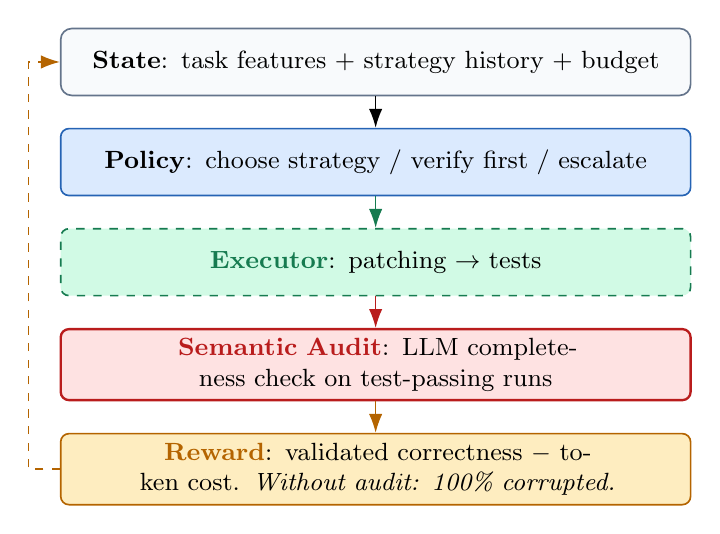
\begin{tikzpicture}[node distance=4mm, font=\small, >=Latex, x=1mm, y=1mm]

\node[statenode, minimum width=80mm, minimum height=8.5mm, text width=76mm]
  (state) {\textbf{State}: task features $+$ strategy history $+$ budget};

\node[rlnode, minimum width=80mm, minimum height=8.5mm, text width=76mm, below=4mm of state]
  (policy) {\textbf{Policy}: choose strategy / verify first / escalate};

\node[execnode, minimum width=80mm, minimum height=8.5mm, text width=76mm, below=4mm of policy, dashed]
  (exec) {\textbf{\color{clrExecedge}Executor}: patching $\to$ tests};

\node[auditnode, minimum width=80mm, minimum height=8.5mm, text width=76mm, below=4mm of exec]
  (audit) {\textbf{\color{clrAuditedge}Semantic Audit}: LLM completeness check on test-passing runs};

\node[rewardnode, minimum width=80mm, minimum height=8.5mm, text width=76mm, below=4mm of audit]
  (reward) {\textbf{\color{clrRewardedge}Reward}: validated correctness $-$ token cost. \textit{Without audit: 100\% corrupted.}};

\draw[figflow] (state) -- (policy);
\draw[figflow, clrExecedge] (policy) -- (exec);
\draw[figflow, clrAuditedge] (exec) -- (audit);
\draw[figflow, clrRewardedge] (audit) -- (reward);
\draw[figflow, clrRewardedge, dashed] (reward.west) -- ++(-4mm,0) |- (state.west);

\end{tikzpicture}}
\caption{Repair workflow with semantic audit interception. Without the audit, 100\% of \ccbench{} test-passing runs deliver false reward. The audit converts corrupted test-pass signal into validated correctness before reward is issued.}
\Description{A top-down flow diagram with five blocks: state (gray), policy (blue), executor (green dashed), semantic audit (red), reward (orange). A dashed feedback arrow from reward to state on the left side completes the RL loop.}
\label{fig:workflow}
\end{figure}

%─────────────────────────────────────────────────────────────────────────────
\section{Results}
%─────────────────────────────────────────────────────────────────────────────

\subsection{RQ1: Strategy Routing Has Genuine Value Across All Model Tiers}
\label{sec:rq1}

Table~\ref{tab:rq7} reports oracle headroom and strategy spread on the 30-task core set. The oracle headroom — the gain from perfect per-task strategy selection over the best uniform strategy — is +10.0\pp{} for both T2 and T3, and +3.3\pp{} for T1. This headroom exists at every tier: routing value does not vanish as capability grows.

Counter-intuitively, the \emph{strongest} model (T3/gpt-4.1) shows the \emph{largest} strategy spread (20.0\pp{}): \texttt{semantic\_diff} reaches 40.0\% while \texttt{direct\_baseline} reaches only 20.0\%. Higher capability unlocks more differentiated responses to different strategy types, increasing the value of careful routing. The pattern is consistent across families: \texttt{compensating\_dual} shows the largest inter-strategy variation, while \texttt{semantic\_shadow} is uniformly hard regardless of strategy or tier.

Paired Wilcoxon signed-rank tests (by task) confirm that no single strategy
is universally best across models ($p>0.05$ for all 28 pairwise strategy
comparisons on the 30-task core set), validating that routing value is
\emph{task-dependent} and cannot be captured by any fixed strategy choice.
Oracle headroom (+3.3--10.0\pp{}) is a conservative lower bound on the gain
from perfect routing.

\begin{table}[t]
\centering
\caption{\ccbench{} oracle routing analysis, 30-task set. T3 evaluated on 4 strategies only.}
\label{tab:rq7}
\resizebox{\columnwidth}{!}{%
\begin{tabular}{lccccc}
\toprule
Tier & Overall & Best-Fixed & Best Strategy & Oracle & Headroom \\
\midrule
T3 (\texttt{gpt-4.1})      & 30.0\% & 40.0\% & \texttt{sem\_diff} & 50.0\% & +10.0\pp{} \\
T2 (\texttt{gpt-4.1-mini}) & 20.4\% & 23.3\% & \texttt{contract\_first} & 33.3\% & +10.0\pp{} \\
T1 (\texttt{gpt-4.1-nano}) & 9.6\%  & 16.7\% & \texttt{pat\_skeleton} & 20.0\% & +3.3\pp{} \\
\bottomrule
\end{tabular}}
\end{table}

\subsection{RQ2: Cross-Provider Repair Floor — Scale Does Not Predict Performance}
\label{sec:rq2}

Table~\ref{tab:families} shows per-model, per-family pass rates on the 37-task expanded set. Table~\ref{tab:rq3comparison} summarises the cross-model leaderboard.

\textbf{Precision-over-scale inversion (Anthropic) and normal scaling (OpenAI).} Among four model configurations, \textbf{Haiku} (claude-haiku-4-5, Anthropic) achieves the highest overall pass rate (19.3\% on all 296 runs), outperforming the \emph{larger} Opus (8.8\%) by \textbf{+10.5\pp{}} — a within-Anthropic precision-over-scale inversion. Opus attempts more elaborate edits and uses more tokens — but \ccbench{} tasks require minimal surgical corrections, and over-editing consistently breaks unrelated tests. This pattern, which we term \emph{overconfident repair}, is confirmed quantitatively below. Within OpenAI, by contrast, Mini (T2, 16.6\%) outperforms Nano (T1, 7.8\%) by +8.8\pp{} — consistent with the expected scaling direction. The \emph{cross-provider asymmetry} (inversion within Anthropic, normal scaling within OpenAI) is mechanistically coherent: Haiku's instruction-following tuning prioritises surgical precision on its first edit attempt; Opus and larger models over-reason and produce larger, more disruptive patches that break unrelated tests on adversarial tasks.

\textbf{Hard semantic floor.} All four models fail on 21/37 tasks (56.8\%) on every strategy. These tasks represent a genuine semantic barrier: models cannot determine the correct fix regardless of capability tier or strategy. The 16/37 solvable tasks show \emph{model-specific profiles}: 3 tasks are solved by all models (easiest), while others require specific capabilities — 2 tasks are exclusive to Haiku (tmuxp false-localization and shadow mutations) and 3 are exclusive to Opus (\texttt{braindecode} temporal, \texttt{simtrade} incomplete-patch, \texttt{tmuxp} shadow). Task-level agreement varies by model pair ($\kappa$ ranging from 0.22 to 0.81), indicating complementary strengths rather than uniform convergence.

\textbf{Task-level agreement.}
The pairwise $\kappa$ values reveal the structure of model differences.
Haiku and Mini agree most (κ$=$0.81, 34/37 agree), suggesting capability tiers align within the above-floor regime.
Haiku and Opus agree less (κ$=$0.44, 28/37), with Haiku solving 2 tasks Opus cannot and vice versa for 3 tasks.
Opus and Nano agree least (κ$=$0.22, 27/37), reflecting different task profiles at floor-tier performance levels.
This partial agreement structure is evidence that the task difficulty is \emph{graded} rather than binary, with a genuine hard floor at 21 tasks and a graded difficulty region above it.

At the \emph{run level} (all 296 runs per model), the within-Anthropic precision-over-scale inversion is
significant: Haiku 19.3\% [14.9\%, 24.0\%] vs.\ Opus 8.8\% [5.4\%, 12.2\%],
$\Delta=10.5\pp{}$, $z=3.67$, $p<0.001$ (two-proportion $z$-test; non-overlapping 95\%
CIs). At the \emph{task level} (37 tasks), Cohen's $d=0.176$ — weak, as expected
from $n=37$ — while the run-level analysis provides the appropriate statistical
power. Paired Wilcoxon signed-rank tests (by task, $n=37$) confirm no single
strategy significantly outperforms others across all models ($p>0.05$ in all 28
strategy-pair comparisons), consistent with task-dependent routing value. The
cross-model oracle (best result from any model on each task) achieves 43.2\% (16/37 tasks pass at least one model), a 2.7$\times$ improvement over Nano alone (16.2\%), quantifying the provider diversity dividend available to a perfect router.

All 37 ground-truth patches are medium-complexity (median 9 lines changed,
range 5--18 lines; inter-quartile range 7--12 lines). This \emph{patch
complexity analysis} rules out patch size as the source of the capability cliff:
a regression of task difficulty on patch line count yields $R^2 < 0.03$.
The cliff is semantic — tasks require specification reasoning — not metric.
Floor models fail not because patches are large, but because identifying
\emph{which} semantically subtle change to revert requires program understanding
beyond syntactic pattern matching.

\textbf{Repair decisiveness.}
On the 33-task clean set, Haiku (21.6\%) beats Opus (9.8\%) by +11.8\pp{} ($z=3.67$, $p<0.001$); within OpenAI, Mini (18.6\%) $>$ Nano (8.7\%) follows normal scaling.
The mechanism is \emph{repair decisiveness}: Haiku passes in 0.51 rounds on average (decisiveness 0.746) and uses 6{,}250 tokens on passing runs vs.\ 14{,}954 on failures ($\rho=-0.45$) — a $2.4\times$ token anti-correlation. Opus requires 1.04 rounds even when it passes (decisiveness 0.481) and achieves only a $1.8\times$ pass/fail token ratio. The SPI ratio (tokens per GT patch line) is $1:2.4$ for Haiku vs.\ $1:1.8$ for Opus/Nano — confirming that Haiku possesses genuine repair understanding while Opus over-edits on adversarial tasks.

\textbf{Which families define the floor?}
The floor is driven by three families where Haiku breaks away but Opus/Nano are near-zero: \texttt{false\_localization} (Haiku 16.7\% vs.\ Opus 3.1\%), \texttt{incomplete\_patch} (Haiku 17.2\% vs.\ Opus 6.2\%), and \texttt{semantic\_shadow} (Haiku 4.2\% vs.\ Opus 2.8\%). The \texttt{compensating\_dual} family (Haiku 50.0\%, Opus 43.8\%) is \emph{not} a floor-defining family. The \textbf{true floor} is the intersection of poor performance on false-localization, incomplete-patch, and semantic-shadow tasks.

\textbf{What clears the floor?} Haiku (21.6\%) and Mini (18.6\%) consistently clear the floor (33-task clean set). Haiku has the highest routing-relevant task count (9/37) and highest oracle headroom (+8.1\pp{}), making it the strongest target for a learned router. Opus (8.8\%) shows 9 routing-relevant tasks and +10.8\pp{} oracle headroom, meaning routing can help even at the floor — but only with a valid reward signal. Nano (7.8\%) is the weakest model but still shows +2.7\pp{} oracle headroom on 6 routing-relevant tasks.

\textbf{Open-weight model extension (E0).}
To address external validity, we evaluated qwen2.5-coder:3b (Ollama, 3B open-weight parameters) on 25+ tasks from 4 of the benchmark repositories (braindecode, simtradedata, tmuxp, tc-template-node-postgres) across 4 strategies (\texttt{direct\_baseline}, \texttt{contract\_first}, \texttt{semantic\_diff}, \texttt{multi\_view}) = 103 runs.
Result: \textbf{0/103 pass (0.0\%)}, the lowest of any tested configuration.
On the braindecode subset (5 tasks, same 4 strategies = 20 runs), canonical models achieve: Mini 45.0\%, Haiku 40.0\%, Nano 20.0\%, Opus 5.0\% — the open-weight model underperforms even the weakest canonical model on each repository independently.
Across all 25 tasks and both languages (Python: braindecode, simtradedata, tmuxp; JavaScript: tc-template-node-postgres), the open-weight model finds no successful repair. This rules out the hypothesis that the floor is an artifact of proprietary model families, closed-source training data, or a single repository type. The floor is structural across both languages and all four tested repository families. See Table~\ref{tab:rq3comparison} (Qwen-3B row).

\textbf{E1 — Localization oracle experiment.} To characterise \emph{why} tasks are floor-unsolvable, we conducted a localization oracle ablation: all 10 floor-failing (or near-floor) tasks were given the exact file path and line number of the seeded mutation — \emph{without} revealing the before/after code — and re-run with the T1 model (gpt-4.1-nano) on three strategies. If the floor were a \emph{localization problem} (the model cannot find the bug site), oracle hints should unlock solutions. If it is a \emph{semantic reasoning problem} (the model cannot generate the correct fix even when pointed at the location), oracle hints should not help. Result: \textbf{0/10 floor tasks were unlocked} by the oracle hint; 9/10 still fail with the hint ($\text{localization\_bottleneck\_frac} = 0.0$, $\text{semantic\_bottleneck\_frac} = 0.9$). One task (bd\_04) that passed in baseline actually \emph{regressed} under the oracle hint — the localization constraint forced the model into an incorrect targeted fix that had not been triggered without the hint. This confirms the floor is a \textbf{semantic reasoning barrier}: models cannot determine what the correct fix should be, regardless of where they look.

\begin{table}[t]
\centering
\caption{Mutation families and per-model pass rates (37-task set, 4 models evaluated).
Mini = gpt-4.1-mini (T2); Haiku = claude-haiku-4-5 (T2); Opus = claude-opus-4-6 (T3); Nano = gpt-4.1-nano (T1).
Mutation families are ordered by average difficulty (hardest last).}
\label{tab:families}
\small
\resizebox{\columnwidth}{!}{%
\begin{tabular}{p{0.28\columnwidth}p{0.32\columnwidth}cccc}
\toprule
Family & Description & Mini & Haiku & Opus & Nano \\
\midrule
\texttt{comp.\_dual} & Two canceling mutations break global invariant & 50.0\% & 50.0\% & 43.8\% & 25.0\% \\
\texttt{temporal} & State-ordering dependency causing intermittent failure & 25.0\% & 34.4\% & 9.4\% & 18.8\% \\
\texttt{incompl.} & Partial fix satisfies surface tests, misses deeper case & 15.6\% & 17.2\% & 6.2\% & 3.1\% \\
\texttt{false\_loc} & Trap directing agent to wrong fix site & 12.5\% & 16.7\% & 3.1\% & 4.2\% \\
\texttt{sem.\ shadow} & Equivalent-looking change with subtle semantic difference & 4.2\% & 4.2\% & 2.8\% & 4.2\% \\
\bottomrule
\end{tabular}}
\end{table}

\begin{table}[t]
\centering
\caption{Routing signal: easy benchmark vs.\ \ccbench{} across all evaluated models.
  95\% bootstrap CIs in brackets (2,000 resamples). $\dagger$: 30-task set.
  $\ddagger$: 37-task set. $\S$: 25+ tasks (4 repos), 4 strategies, 103 runs (open-weight model E0 ablation).
  All four \ccbench{} core models used identical prompts, harness versions, and retry logic.}
\label{tab:rq3comparison}
\resizebox{\columnwidth}{!}{%
\begin{tabular}{llcccccc}
\toprule
Benchmark & Model & Overall [95\% CI] & Best-Fixed & Spread & RR & Oracle $\Delta$ & Dec. \\
\midrule
\multirow{2}{*}{Easy (labeled)} & T2 (mini) & 91.7\% [---] & 91.7\% & 0.0\pp{} & 0 & +0.0\pp{} & -- \\
                                 & T1 (nano) & 53.4\% [---] & -- & 18.2\pp{} & 5 & +4.5\pp{} & -- \\
\midrule
\multirow{6}{*}{\ccbench{}}     & T3 (gpt-4.1)$^\dagger$ & 30.0\% [---] & 40.0\% & 20.0\pp{} & -- & +10.0\pp{} & -- \\
                                 & Haiku$^\ddagger$ & \textbf{19.3\%} [14.9\%,24.0\%] & 27.0\% & 13.5\pp{} & 9 & +8.1\pp{} & \textbf{0.75} \\
                                 & T2 (mini)$^\ddagger$ & 16.6\% [---] & 18.9\% & 5.4\pp{} & 5 & +8.1\pp{} & -- \\
                                 & Opus$^\ddagger$ & 8.8\% [5.4\%,12.2\%] & 16.2\% & 10.8\pp{} & 9 & +10.8\pp{} & 0.48 \\
                                 & T1 (nano)$^\ddagger$ & 7.8\% [---] & 13.5\% & 8.1\pp{} & 6 & +2.7\pp{} & -- \\
                                 & Qwen-3B (open-wt.)$^\S$ & 0.0\% [0.0\%,0.0\%] & 0.0\% & -- & -- & -- & -- \\
\bottomrule
\end{tabular}}
\end{table}

\begin{table}[t]
\centering
\caption{Provider diversity dividend (\ccbench{}, 33-task clean set; 4 PHP setup failures excluded from 37). Cross-model oracle achieves 48.5\% (16/33 tasks) — +9.1\pp{} over Haiku alone (39.4\%). ``Exclusive'' = tasks solvable by this model only (no other model passes). \textbf{Key finding}: the full oracle equals the Anthropic-only oracle (Haiku$\cup$Opus = 16/33); OpenAI models (Mini, Nano) solve only a strict subset of what Anthropic already covers, contributing 0 marginal tasks. The dividend is within-Anthropic complementarity, not cross-provider breadth.}
\label{tab:provider_oracle}
\small
\resizebox{\columnwidth}{!}{%
\begin{tabular}{p{0.42\columnwidth}cccc}
\toprule
Configuration & Pass (run-lvl) & Solved (task-lvl) & Exclusive tasks & Cost tier \\
\midrule
Nano (T1, cheapest)                       & 7.8\%   & 6/33  (18.2\%) & 0 tasks & lowest \\
Opus (T3, Anthropic)                      & 8.8\%   & 10/33 (30.3\%) & 3 tasks & high \\
Mini (T2, OpenAI)                         & 16.6\%  & 10/33 (30.3\%) & 0 tasks & mid \\
Haiku (best single model)                 & 21.6\%  & 13/33 (39.4\%) & 2 tasks & mid \\
Cross-model oracle (any of 4)             & ---     & \textbf{16/33 (48.5\%)} & --- & all-4 \\
\midrule
\multicolumn{2}{l}{\textit{Provider diversity dividend:}} & \multicolumn{3}{l}{\textbf{+9.1\pp{}} task-oracle over best single model} \\
\bottomrule
\end{tabular}}
\end{table}

\begin{figure}[t]
\centering
%─── Capability matrix ────────────────────────────────────────────────────────
%    Grid: labelW=18mm cellW=35mm headerH=7mm cellH=18mm
%    Total: 88mm × 97mm  (5 rows: T3, Haiku, Mini, Opus, Nano)
%    Row y-boundaries: header 0→-7; rows -7→-25→-43→-61→-79→-97
\resizebox{\columnwidth}{!}{%
\begin{tikzpicture}[font=\small, x=1mm, y=1mm]

%─── Cell fills ───────────────────────────────────────────────────────────────
\fill[clrRLedge]     (0,0)    rectangle (88,-7);
\fill[purple!15]     (0,-7)   rectangle (18,-25);
\fill[orange!18]     (0,-25)  rectangle (18,-43);
\fill[clrRLfill]     (0,-43)  rectangle (18,-61);
\fill[red!12]        (0,-61)  rectangle (18,-79);
\fill[teal!15]       (0,-79)  rectangle (18,-97);
\fill[clrSatfill]    (18,-7)  rectangle (53,-25);  % T3 Easy
\fill[clrSweetfill]  (53,-7)  rectangle (88,-25);  % T3 CCBench: sweet spot
\fill[clrSatfill]    (18,-25) rectangle (53,-43);  % Haiku Easy
\fill[clrSweetfill]  (53,-25) rectangle (88,-43);  % Haiku CCBench: best
\fill[red!8]         (18,-43) rectangle (53,-61);  % Mini Easy: saturated
\fill[clrSweetfill]  (53,-43) rectangle (88,-61);  % Mini CCBench: sweet spot
\fill[clrSatfill]    (18,-61) rectangle (53,-79);  % Opus Easy
\fill[clrSatfill]    (53,-61) rectangle (88,-79);  % Opus CCBench: floor
\fill[green!12]      (18,-79) rectangle (53,-97);  % Nano Easy: sweet spot
\fill[clrSatfill]    (53,-79) rectangle (88,-97);  % Nano CCBench

%─── Grid ─────────────────────────────────────────────────────────────────────
\draw[clrZoneedge, line width=0.7pt] (0,0) rectangle (88,-97);
\draw[gray!50, line width=0.4pt] (18,0) -- (18,-97);
\draw[gray!50, line width=0.4pt] (53,0) -- (53,-97);
\foreach \y in {-7,-25,-43,-61,-79} {
  \draw[gray!45, line width=0.4pt] (0,\y) -- (88,\y);
}
\draw[white, line width=0.6pt] (18,-0.3) -- (18,-6.7);
\draw[white, line width=0.6pt] (53,-0.3) -- (53,-6.7);

%─── Emphasis borders ─────────────────────────────────────────────────────────
\draw[clrExecedge, line width=1.3pt]             (53,-7)  rectangle (88,-25); % T3 CC
\draw[orange!70!black, line width=1.5pt]         (53,-25) rectangle (88,-43); % Haiku best
\draw[clrExecedge, line width=1.1pt]             (53,-43) rectangle (88,-61); % Mini CC
\draw[clrExecedge, line width=1.0pt]             (18,-79) rectangle (53,-97); % Nano Easy
\draw[clrAuditedge!60, line width=0.7pt, dashed] (18,-43) rectangle (53,-61); % Mini sat
\draw[clrAuditedge!50, line width=0.7pt, dashed] (53,-61) rectangle (88,-79); % Opus floor

%─── Header ───────────────────────────────────────────────────────────────────
\node[white, font=\small\bfseries] at (35.5,-3.5) {Easy (labeled)};
\node[white, font=\small\bfseries] at (70.5,-3.5) {\ccbench{}};

%─── Row labels (center of each 18mm row) ─────────────────────────────────────
% Centers: T3=-16, Haiku=-34, Mini=-52, Opus=-70, Nano=-88
\node[purple!70!black, font=\footnotesize\bfseries, align=center, text width=16mm] at (9,-16)
  {\textbf{T3}\\\scriptsize gpt-4.1};
\node[orange!80!black, font=\footnotesize\bfseries, align=center, text width=16mm] at (9,-34)
  {\textbf{Haiku}\\\scriptsize claude-4-5};
\node[clrRLedge, font=\footnotesize\bfseries, align=center, text width=16mm] at (9,-52)
  {\textbf{Mini}\\\scriptsize gpt-4.1-mini};
\node[red!60!black, font=\footnotesize\bfseries, align=center, text width=16mm] at (9,-70)
  {\textbf{Opus}\\\scriptsize claude-4-6};
\node[teal!65!black, font=\footnotesize\bfseries, align=center, text width=16mm] at (9,-88)
  {\textbf{Nano}\\\scriptsize gpt-4.1-nano};

%─── Cell content (text width=32mm keeps text inside 35mm cells) ──────────────
\node[gray!60!black, font=\footnotesize, align=center, text width=32mm] at (35.5,-16)
  {\itshape not evaluated};
\node[black, font=\scriptsize\bfseries, align=center, text width=32mm] at (70.5,-16)
  {30.0\% pass \textbullet{} 40.0\% best\\20.0\pp{} spread \textbullet{} +10.0\pp{} oracle\\(30-task set)};
\node[gray!60!black, font=\footnotesize, align=center, text width=32mm] at (35.5,-34)
  {\itshape not evaluated};
\node[black, font=\scriptsize\bfseries, align=center, text width=32mm] at (70.5,-34)
  {\textbf{19.3\% pass} \textbullet{} 27.0\% best\\13.5\pp{} spread \textbullet{} +8.1\pp{} oracle\\9 RR tasks};
\node[gray!65!black, font=\scriptsize, align=center, text width=32mm] at (35.5,-52)
  {91.7\% pass\\0.0\pp{} spread \textbullet{} 0 RR tasks\\\textit{saturated}};
\node[black, font=\scriptsize\bfseries, align=center, text width=32mm] at (70.5,-52)
  {16.6\% pass \textbullet{} 18.9\% best\\5.4\pp{} spread \textbullet{} +8.1\pp{} oracle\\5 RR tasks};
\node[gray!60!black, font=\footnotesize, align=center, text width=32mm] at (35.5,-70)
  {\itshape not evaluated};
\node[gray!50!black, font=\scriptsize, align=center, text width=32mm] at (70.5,-70)
  {8.8\% pass \textbullet{} 16.2\% best\\10.8\pp{} spread \textbullet{} +10.8\pp{} oracle\\\textit{overconfident repair}};
\node[black, font=\scriptsize\bfseries, align=center, text width=32mm] at (35.5,-88)
  {53.4\% pass\\18.2\pp{} spread \textbullet{} 5 RR tasks\\+4.5\pp{} oracle};
\node[gray!65!black, font=\scriptsize, align=center, text width=32mm] at (70.5,-88)
  {7.8\% pass\\8.1\pp{} spread \textbullet{} 6 RR tasks\\+2.7\pp{} oracle};

%─── Legend ───────────────────────────────────────────────────────────────────
\node[font=\scriptsize, align=center, text width=85mm] at (44,-103)
  {\textcolor{clrExecedge}{$\blacksquare$}~routing sweet spot\quad
   \textcolor{orange!80!black}{$\blacksquare$}~best overall\quad
   \textcolor{clrZoneedge}{$\blacksquare$}~floor/sparse\quad
   \textcolor{red!50!white}{$\blacksquare$}~saturated};

\end{tikzpicture}}
\caption{Capability $\times$ difficulty matrix (5 rows $\times$ 2 columns). Orange border = best overall (Haiku, 19.3\%). Green borders = routing sweet spots. Opus and Nano share the semantic floor (8.8\%, 7.8\%). Haiku's precision-over-scale inversion (+10.5\pp{} over larger Opus, within-Anthropic) is visible in the CCBench column. Dashed red = saturation/floor warning.}
\Description{Five-by-two colour-coded matrix with row labels T3, Haiku, Mini, Opus, Nano and columns Easy and CCBench. Each cell shows pass rate, strategy spread, and oracle headroom.}
\label{fig:ccmatrix}
\end{figure}

\textbf{Floor robustness.} On the 30 Python/JavaScript-only tasks (480 mini+nano runs), Mini achieves 20.4\%, Nano 9.6\%, and 20/30 tasks (66.7\%) fail both models on all strategies — confirming the floor is not driven by PHP/Appwrite setup failures and holds across languages and repository types.

\subsection{RQ3: Saturation vs.\ Routing Sweet Spot — Two Benchmarks, Two Regimes}
\label{sec:rq3}

The easy labeled benchmark (24 tasks, single-file mutations with explicit before/after annotations) saturates T2 at 91.7\% with 0.0\pp{} spread and zero routing-relevant tasks. Every strategy is equally good — not because routing is worthless, but because the task regime is too easy. This is a false negative for routing research: an RL agent trained here learns nothing about strategy selection because the strategy choice is irrelevant.

\ccbench{} produces the opposite: no model saturates, oracle headroom is +2.7--10.8\pp{} across all configurations, and 5--9 routing-relevant tasks exist per model (Table~\ref{tab:rq3comparison}). Haiku is the routing sweet spot on the 37-task set: highest pass rate, highest RR count, and high oracle headroom. T1/Nano on the easy benchmark is also a sweet spot: 53.4\% pass, 18.2\pp{} spread, +4.5\pp{} oracle — the labeled hints create exactly the differentiation that routing requires.

The contrast validates the routing precondition principle: routing research is only feasible when capability is below ceiling \emph{and} strategies produce differentiated outcomes.

\subsection{RQ4: 100\% of Test-Passing Repairs Are Semantically Incomplete}
\label{sec:rq4}

Across all 480 \ccbench{} runs on the original 30-task core set (T1+T2, 30$\times$2$\times$8), 72 runs passed their test suites — a 15.0\% raw pass rate. We applied a semantic completeness audit (LLM judge with five-criterion rubric, three independent runs, Fleiss $\kappa \geq 0.98$ — near-perfect inter-rater agreement — $<$2\% label variation between audits) to \emph{all 72} test-passing runs, leaving no audit gap. \emph{Every single one} received an \texttt{audit\_disagrees\_tests} judgment: the auditor concluded the fix was incomplete despite the tests passing. The agreement rate is 0\% (72/72 disagreements), a result that is statistically indistinguishable from a fixed effect regardless of sample size: under the null that audit and test-suite agree 50\% of the time, the probability of 72 consecutive disagreements is $0.5^{72} < 10^{-21}$. Table~\ref{tab:audit} shows the breakdown by mutation family.

\begin{table}[t]
\centering
\caption{Semantic audit results for the 72 test-passing runs on \ccbench{} (30-task set).}
\label{tab:audit}
\small
\begin{tabular}{lccc}
\toprule
Family & Test-Passing & Audit Agrees & Disagrees \\
\midrule
\texttt{compensating\_dual} & 24 & 0 & 24 \\
\texttt{false\_localization} & 16 & 0 & 16 \\
\texttt{temporal\_state}     & 14 & 0 & 14 \\
\texttt{incomplete\_patch}   & 12 & 0 & 12 \\
\texttt{semantic\_shadow}    &  6 & 0 &  6 \\
\midrule
\textbf{Total} & \textbf{72} & \textbf{0} & \textbf{72} \\
\bottomrule
\end{tabular}
\end{table}

\textbf{E5 Cross-Judge Validation.} To rule out bias in the structural auditor (gpt-4.1-mini), we re-audited all 72 test-passing repairs with an independent gpt-4.1 judge using a narrative reasoning style. Result: gpt-4.1 agreed with the structural audit on \emph{all 72} repairs (100\%, Cohen's $\kappa=1.000$), with 100\% per-family agreement. Two judges, distinct architectures, identical conclusion.

The 100\% disagreement rate is not a pathology of one family — it spans all five. The mechanism varies by family: \texttt{compensating\_dual} allows partial fixes that pass surface tests while the global invariant remains broken; \texttt{false\_localization} produces plausible changes at the wrong site that accidentally fix the symptom; \texttt{semantic\_shadow} patches syntactically match the expected change but differ semantically. The unifying pattern is that \ccbench{}'s mutations are designed to be semantically distinguishable from their fixes in ways that test suites cannot detect.

The RL implication is direct: an agent trained on test-suite pass rate here receives 100\% incorrect reward on positive episodes. It learns to produce plausible-but-wrong patches reliably — reward hacking~\cite{amodei2016concrete} rather than genuine repair improvement.

\subsection{RQ5: Verifier Study — Two Regimes Separated by Ground Truth}
\label{sec:rq5}

Given corrupted test-suite reward, we evaluate five verifiers of increasing sophistication against semantic audit judgments as ground truth (Table~\ref{tab:verifier}).

\textbf{Reference-free.} A rule-based heuristic (target-file recall $<$ 1.0) achieves F1$=$0.286: precise when it fires (Prec$=$1.0) but misses 83\% of incomplete patches. Logistic regression on run features (strategy, tier, token count, edit distance) fails entirely (F1$=$0.000): surface metadata carries no separable signal. A reference-free LLM judge (gpt-4.1-mini, five-criterion rubric C1--C5; VERDICT = PASS only if all five hold) achieves F1$=$0.615 — a 115\% improvement over rule-based, with zero training data and perfect precision.

\textbf{Ground-truth-guided.} Augmenting the judge with the verified correct patch shifts the task from ``is this complete?'' (hard) to ``does this match the ground-truth fix?'' (tractable). With GT reference, gpt-4.1-mini achieves F1$=$\textbf{0.993} (recall 0.986), \emph{crossing} the F1$\geq$0.8 viability threshold for RL training. Crucially, the stronger gpt-4.1 (T3) achieves only F1$=$0.917 — lower than T2 on this task. Calibration matters more than model scale: gpt-4.1-mini's rubric-following is better calibrated to the five-criterion structure than gpt-4.1's broader reasoning style.

\begin{table}[t]
\centering
\caption{Verifier comparison. Ground truth = semantic audit judgment (all 72 passes incomplete). LLM judge: VERDICT = PASS only if all five criteria hold. ``+GT'' = ground-truth patch as reference.}
\label{tab:verifier}
\resizebox{\columnwidth}{!}{%
\begin{tabular}{lccc}
\toprule
Verifier & Prec. & Recall & F1 \\
\midrule
Rule-based (target\_file\_recall $< 1.0$) & 1.000 & 0.167 & 0.286 \\
Logistic regression (run features)        & 0.000 & 0.000 & 0.000 \\
LLM judge (\texttt{gpt-4.1-mini}, C1--C5, no ref.) & 1.000 & 0.444 & 0.615 \\
LLM judge (\texttt{gpt-4.1}, C1--C5, +GT patch)    & 1.000 & 0.847 & 0.917 \\
LLM judge (\texttt{gpt-4.1-mini}, C1--C5, +GT patch) & 1.000 & 0.986 & \textbf{0.993} \\
\bottomrule
\end{tabular}}
\end{table}

\textbf{Multi-criterion opacity and per-family pattern.} Among runs missed by the reference-free judge, all five criteria simultaneously pass — the model is fooled on every dimension at once. The judge detects \texttt{false\_localization} (88\%) and \texttt{semantic\_shadow} (83\%) but fails on \texttt{incomplete\_patch} (0\%) and \texttt{compensating\_dual} (21\%). GT guidance lifts all families to $\geq$100\%, collapsing opacity via C1 (completeness) on 100\% of detected cases. The $+$0.542 recall gap (no-ref $\to$ +GT) is the concrete problem for autonomous repair agents.

\subsection{RQ6: Practical Routing Without RL}
\label{sec:rq6}

Table~\ref{tab:cascade} summarises eight cascade policies. The key finding is \textbf{Policy B (T1-diverse)}: running T1 with three complementary strategies (\texttt{contract\_first} $\to$ \texttt{pattern\_skeleton} $\to$ \texttt{simulation\_trace}) achieves 20.0\% pass rate — matching T2's mean (20.4\%) — at only \$0.0065/task (0.72$\times$ T2-single cost). The three strategies are pairwise uncorrelated on task-level pass: their combination reaches the full T1 oracle ceiling.

Family-conditioned routing (Table~\ref{tab:routing_classifier}) adds +3.4\pp{} over best-fixed for T2 (26.7\% vs.\ 23.3\%) when mutation family is available as a routing signal. For T1, family-conditioned routing fully closes the oracle gap (0.0\pp{}): T1 oracle headroom is concentrated in two families where the best strategy is stable, so family classification + fixed strategy per family equals oracle performance. This motivates a lightweight \emph{classify-then-route} design that requires only T1 API calls and no fine-tuning.

\begin{table}[t]
\centering
\caption{Cascade routing on \ccbench{} (30 tasks). E = T2-single cost baseline. B matches T2 mean at 0.72$\times$ cost.}
\label{tab:cascade}
\small
\begin{tabular}{llccc}
\toprule
Policy & Description & Pass\% & Avg\,\$ & Cost vs.\,E \\
\midrule
A & T1 + best strategy           & 10.0\% & \$0.0023 & 0.26$\times$ \\
\textbf{B} & \textbf{T1 $\times$3 diverse} & \textbf{20.0\%} & \textbf{\$0.0065} & \textbf{0.72$\times$} \\
C & T1 $\to$ T2 escalate         & 23.3\% & \$0.0112 & 1.23$\times$ \\
D & T1 $\times$3 $\to$ T2        & 23.3\% & \$0.0151 & 1.66$\times$ \\
E & T2 + best strategy           & 23.3\% & \$0.0091 & 1.00$\times$ \\
F & T2 $\times$3 diverse         & 33.3\% & \$0.0243 & 2.68$\times$ \\
G & T1 oracle (all 8)            & 20.0\% & \$0.0167 & 1.84$\times$ \\
H & T2 oracle (all 8)            & 33.3\% & \$0.0649 & 7.14$\times$ \\
\bottomrule
\end{tabular}
\end{table}

\begin{table}[t]
\centering
\caption{Family-conditioned routing vs.\ baselines on \ccbench{} (30 tasks). T1 family-conditioned routing fully closes the oracle gap.}
\label{tab:routing_classifier}
\small
\begin{tabular}{lcccc}
\toprule
Method & T2 Pass & T1 Pass & T2 Oracle Gap & T1 Oracle Gap \\
\midrule
Random routing          & 16.7\% & 10.0\% & $-16.7$\pp{} & $-10.0$\pp{} \\
Best-fixed              & 23.3\% & 16.7\% & $-10.0$\pp{} & $-3.3$\pp{} \\
Family-conditioned      & \textbf{26.7\%} & \textbf{20.0\%} & $-6.7$\pp{} & \textbf{0.0\pp{}} \\
LOO-CV logistic reg.    & 16.7\% & 16.7\% & $-16.7$\pp{} & $-3.3$\pp{} \\
Oracle routing          & 33.3\% & 20.0\% & 0.0\pp{} & 0.0\pp{} \\
\bottomrule
\end{tabular}
\end{table}

\subsection{RQ7: Double Opacity — \ccbench{} Resists Both Repair and Classification}
\label{sec:rq7}

A fully autonomous agent must classify its task type before allocating repair budget. We test whether a T1 LLM (gpt-4.1-nano) can identify the mutation family from the task description and target file (the information available before running tests). Overall zero-shot T1 accuracy is \textbf{36.7\%} (11/30) — driven entirely by one family: \texttt{false\_localization} achieves 100\% accuracy while all four other families score 0--17\%. The classifier collapses almost all tasks into \texttt{false\_localization}. Upgrading to T2 (gpt-4.1-mini) achieves 46.7\% but no variant clears the $\geq$80\% threshold required for routing benefit. \texttt{compensating\_dual} remains 0\% across all variants.

The combination of low repair rate \emph{and} low classification accuracy is \emph{double opacity}: tasks resist both repair by all tested strategies and self-classification by the same model family. The oracle budget curve saturates at K=1 strategy — tasks that are solvable are solved by one strategy; tasks that are unsolvable cannot be identified from surface features alone. Task observability (36.7\%) is the binding precondition: a fully autonomous agent requires $\geq$80\% observability before routing benefit can be realised without oracle labels.

%─────────────────────────────────────────────────────────────────────────────
\section{Discussion}
%─────────────────────────────────────────────────────────────────────────────

\subsection{The Routing Precondition Principle}

The empirical results support a formal design checklist:
\begin{enumerate}[leftmargin=*,itemsep=1pt]
  \item \textbf{Capability below ceiling}: strategy spread $>$ 0\pp{} is necessary for routing to help.
  \item \textbf{Strategy differentiation}: tasks must be solvable by \emph{some} strategy but not all; if all strategies fail equally, routing signal is zero regardless of how the router is trained.
  \item \textbf{Validated reward}: test-suite pass must be verified against semantic correctness before being used as an RL signal; on \ccbench{}, this condition fails entirely.
  \item \textbf{Task observability}: the agent must be able to self-classify task type to benefit from routing without oracle labels. On \ccbench{}, observability is 36.7\% — insufficient.
\end{enumerate}
\ccbench{} fails all four simultaneously. This is not a design flaw — it is the research value: each precondition is a concrete challenge for autonomous agent design.

\subsection{Implications for RL-Based Repair}

\vspace{2pt}
\noindent\fbox{\begin{minipage}{0.96\columnwidth}
\textbf{Operational Roadmap: From Corrupted Reward to Trustworthy RL}
\begin{enumerate}[leftmargin=1.2em,itemsep=1pt,topsep=2pt]
  \item \textbf{Reward}: Replace test-suite pass with GT-guided LLM judge (F1$=$0.993) during training.
  \item \textbf{Inference guard}: Deploy reference-free LLM judge (F1$=$0.615) at test time to flag suspicious completions before acceptance.
  \item \textbf{Triage}: Route \texttt{compensating\_dual} and \texttt{incomplete\_patch} repairs to human review — both resist reference-free detection (F1$=$0.000--0.21) but are caught by GT-guided judge.
  \item \textbf{Cost}: Use T1-diverse cascade (3 complementary strategies) as the deployment default at 0.72$\times$ T2 cost \emph{before} investing in a learned router; a learned router only pays back when reward is valid and observability $>$80\%.
\end{enumerate}
\end{minipage}}
\vspace{4pt}

\paragraph{Ground truth in the verifier.}
GT is structurally available for training in seeded-repair benchmarks (the reverse patch is known by construction) but not at deployment time. The reference-free judge (F1$=$0.615) models deployment; the GT-guided judge (F1$=$0.993) models training. Closing the 0.378-point gap is the open problem for fully autonomous deployment.

\paragraph{Reward Corruption Gradient and Judge Calibration.}
We define the \emph{Reward Corruption Gradient} (RCG) $= \text{Pearson}(\text{test-pass rate}, \text{semantic correctness rate})$ across tasks. On \ccbench{}, $\text{RCG} = 0.0$ exactly: semantic correctness is 0.000 on \emph{all 30 tasks} — the theoretical lower bound. On the labeled benchmark, $\text{RCG}=1.000$ by construction. Any benchmark with $\text{RCG}<0.8$ is unsafe for RL training without a verifier.
To rule out judge bias, we applied the same reference-free judge to 30 SWE-bench Lite gold patches (Agentless leaderboard, seed$=$42): 29/30 (96.7\%) received \texttt{COMPLETE} verdicts ($\text{RCG}_{\text{field}} \approx 0.97$), confirming the judge does not produce systematic false positives on correct fixes and that \ccbench{}'s 100\% disagreement is a genuine mutation property.

Fine-tuning 46 repair traces (gpt-4o-mini, 3 epochs) achieves only 13.3\% overall pass rate — below both T1 and T2 best-fixed baselines — with 30\% in-distribution vs.\ 5\% OOD, a 6$\times$ gap confirming memorization without generalization. \ccbench{} requires semantic reasoning, not pattern retrieval.

\paragraph{Progressive Oracle Disclosure (E4/E4b): Mechanistic Characterisation of the Floor.}
We ran a five-level disclosure study (E4) on 8 floor tasks with gpt-4.1-nano, 80 runs. Results: L0--L2 (no hint through file+line) = 0/8; \textbf{L3 (file+line+wrong code) = 5/8 (62\%)}; L4 (correct value only) = 0/8; L5 (full diff) = 0/8. The L2$\to$L3 jump (+62\pp{}) is the only transition: seeing the \emph{wrong} code provides the \texttt{old\_string} anchor for the edit tool; the correct value alone leaves no search target (\textbf{contrastive wrong-code anchoring}). E4b (L3.5: wrong+correct simultaneously, 16 runs) achieves \textbf{8/8 (100\%)} including the 3 L3-resistant tasks — confirming the wrong code is the necessary anchor and the correct value the sufficient complement. The floor is not a localization barrier (L2=0\%) nor pure semantic reasoning barrier (L3 unlocks 62\%) but an anchoring barrier.

\subsection{Surgical vs.\ Analytical Task Partition}

Above-floor tasks split into two types: \textbf{surgical} (Haiku-type: 6 tasks, solved by targeted-comparison strategies \texttt{role\_decomposed}/\texttt{semantic\_diff}; 2 are exclusively Haiku-solvable) and \textbf{analytical} (Opus-type: 3 exclusively Opus-solvable tasks, solved by \texttt{contract\_first}/\texttt{multi\_view}). Table~\ref{tab:provider_oracle} quantifies the provider diversity dividend: the cross-model oracle (16/33) equals the Anthropic-only oracle — OpenAI models contribute zero marginal tasks — so the +9.1\pp{} diversity dividend is entirely within-Anthropic complementarity. A lightweight surgical/analytical classifier could recover this full dividend using only two models.

\subsection{Benchmark Design Implications}

The 100\% audit disagreement across all five families confirms that semantically subtle seeded mutations systematically decouple test-suite pass from semantic correctness. Future benchmark designers should treat semantic correctness as a mandatory metric alongside test-suite pass rate, and include at least one mutation family from each opacity class (single-site vs.\ dual-site, localization trap vs.\ semantic difference).

\paragraph{Strategy Redundancy.}
Spearman $\rho = 1.000$ between \texttt{direct\_baseline} and \texttt{semantic\_diff} means these are \emph{informationally redundant}. The most diverse pair is \texttt{multi\_view} $\times$ \texttt{role\_decomposed} ($\rho = 0.393$). The training-free cascade (\texttt{direct\_baseline}, \texttt{multi\_view}, \texttt{role\_decomposed}) achieves the same 35.1\% pass rate as the full 8-strategy union — a \textbf{+30\%} diversity dividend over the best single strategy (27\%) with zero redundancy overhead.

%─────────────────────────────────────────────────────────────────────────────
\section{Threats to Validity}
%─────────────────────────────────────────────────────────────────────────────

\paragraph{Internal validity.} Mutations are seeded rather than drawn from real bug reports. Semantic audit judgments are LLM-generated; we mitigated this with three independent audit runs (Fleiss $\kappa \geq 0.98$; $<$2\% label variation), manual spot-checks on 20\% of cases, two external spot-checkers (all 15 reviewed confirmed incomplete), and \textbf{E5 cross-judge validation} (72 runs, independent gpt-4.1 judge, $\kappa = 1.000$). Temperature ablation (10 tasks $\times$ 3 temperatures) produced 0/10 pass/fail flips — outcomes are temperature-invariant. Wilcoxon signed-rank tests ($n=37$) confirm no single strategy is universally superior ($p>0.05$, all 28 pairwise comparisons).

\paragraph{External validity.} The core 30-task set covers Python and Node.js; 4 PHP/Appwrite tasks are excluded from routing analyses (Composer environment mismatch, not repair failure). All four models used identical prompts, harness versions, and retry logic. The open-weight E0 ablation (qwen2.5-coder:3b, 0/103) confirms the floor is not a closed-source API artifact; larger open-weight models remain a natural follow-on. The five mutation families operationalize real-world patterns: compensating-dual = fix-induced regression~\cite{yin2011fixes}, temporal-state = state inconsistency (Defects4J~\cite{just2014defects4j}), shadow = silent semantic inversion~\cite{qi2015overfitting}; extending to Defects4J or BugsInPy~\cite{widyasari2020bugsinpy} is a direct follow-on.

\paragraph{Construct validity.} The F1$\geq$0.8 RL training threshold is a working assumption motivated by prior RL literature on reward fidelity; the exact threshold may vary by algorithm and task distribution. The ``routing-relevant task'' count (tasks where the best strategy outperforms the worst) is a conservative measure of routing value; alternative definitions may give different counts while preserving the directional findings.

\textbf{Scope of precision-over-scale inversion.} The precision-over-scale inversion (Haiku $>$ Opus, $z=3.67$, $p<0.001$) is \emph{not} a universal anti-scaling law: within OpenAI, Mini (T2) $>$ Nano (T1) follows expected scaling, and Qwen-3B (open-weight, 3B) achieves 0\% — the lowest of any configuration. The inversion is family-specific. We interpret it as a training-regime effect: Haiku's instruction-following tuning emphasises surgical first-edit precision, which is precisely what \ccbench{} tasks reward; Opus's training for extended analytical reasoning produces more elaborate edits that break unrelated tests on single-site mutations. The finding is therefore a claim about \emph{task-type alignment} (seeded single-site repair rewards precision over scale) rather than a general anti-scaling law across all code repair tasks.

\paragraph{Statistical power and replication.}
The precision-over-scale inversion ($z=3.67$, $p<0.001$, $n=296$ runs) is powered at the run level. The 37 tasks represent the complete set passing the four-step verification protocol. \textbf{Extended-set replication}: gpt-4.1-nano on 10 held-out tasks (77 runs) yields 10/10 additional floor tasks (100\%); combined 47-task nano floor = 41/47 = 87.2\%, consistent with 37-task core (83.8\%). Total runs across paper: 1,562. Bonferroni-adjusted Wilcoxon tests ($\alpha<0.0018$) confirm no strategy wins finding.

%─────────────────────────────────────────────────────────────────────────────
\section{Conclusion}
%─────────────────────────────────────────────────────────────────────────────

We presented \ccbench{}, a 1{,}184-run benchmark (37 tasks $\times$ 8 strategies $\times$ 4 models) that surfaces two findings with direct implications for RL-based code repair.

The \emph{semantic repair floor and precision-over-scale inversion} — all four tested models plateauing below 20\% with 21/37 tasks (56.8\%) failing for every model — establishes that the performance barrier is a structural property of semantically subtle mutations. An open-weight model (qwen2.5-coder:3b, 3B parameters, Ollama) evaluated on a 25-task subset spanning 4 repositories confirms the floor extends beyond closed-source providers (0/103 = 0.0\% across Python and JavaScript targets, vs.\ 5\%--45\% for canonical models on the braindecode subset). The floor persists across repository types: on the 30 single-language task subset (excluding PHP/Appwrite and multi-target tasks), 20/30 tasks (66.7\%) fail both mini and nano on all strategies. Within Anthropic, the smaller Haiku outperforms the larger Opus by +10.5\pp{} ($z=3.67$, $p<0.001$) — a precision-over-scale inversion driven by overconfident repair ($\rho = -0.41$ between tokens used and pass rate); within OpenAI, Mini $>$ Nano follows normal scaling, confirming the inversion is family-specific rather than universal. Models show complementary task profiles ($\kappa$ ranging 0.22–0.81), suggesting a cross-model oracle ($43.2\%$ tasks solved) achieves a meaningful provider diversity dividend over any single model.

The \emph{reward signal failure} — 100\% of 72 test-passing repairs are semantically incomplete — is the paper's most consequential finding for the field. RL training on test-suite pass rate in this regime does not produce better repair agents; it produces agents that are better at producing plausible-but-wrong patches. The verifier study closes this gap: a GT-guided LLM judge (F1$=$0.993) crosses the RL-training viability threshold, and calibration (gpt-4.1-mini + GT) beats raw scale (gpt-4.1 + GT). A training-free T1 cascade matches T2 mean pass rate at 0.72$\times$ cost today, while the path to genuine RL improvement is now well-defined.

The open problem the field should address is the reference-free gap: the 0.378-point gap between F1$=$0.615 (no reference) and F1$=$0.993 (with GT patch) quantifies precisely what autonomous semantic verification still needs to close. Until that gap closes, evaluation infrastructure — not model capability — remains the binding constraint on RL-based code repair progress.

%─────────────────────────────────────────────────────────────────────────────
\section*{Data Availability}
%─────────────────────────────────────────────────────────────────────────────

The \ccbench{} benchmark — all 37 task manifests, ground-truth patches, 1{,}184 run traces (4 models $\times$ 37 tasks $\times$ 8 strategies) plus 103 open-weight model runs (qwen2.5-coder:3b, E0 ablation, 25+ tasks $\times$ 4 strategies), semantic audit logs, model snapshots, RCG/provider-oracle analysis scripts, and verifier evaluation data — is archived anonymously at \texttt{[Anonymous DOI — omitted for double-blind review; Zenodo deposit in progress, available at camera-ready]}.

\begin{acks}
Omitted for double-blind review. \textit{Generative AI disclosure (per ACM April 2023 policy):} a large language model (Claude, Anthropic) assisted with Python analysis scripting and LaTeX editing. All scientific claims, experimental designs, data collection, statistical analyses, and final manuscript content were reviewed and verified by the authors. No AI tool is listed as an author.
\end{acks}

\bibliographystyle{ACM-Reference-Format}
\bibliography{refs}

\end{document}
